\chapter{Popis implementace}
V této kapitole si představíme klíčové a zajímavé části implementace. Pro více detailů o implementaci je možné nahlédnout do kódu, který obsahuje dokumentační komentáře.

Pro celý projekt používáme jedno C\# solution. To obsahuje dva C\# projekty. Prvním je hra (\texttt{WorldSimulator.csproj}) a druhým je měření (\texttt{WorldSimula-} \texttt{tor.Benchmarks.csproj}), které používá vytvořenou hru pro měření výkonu ECS knihoven. Projekt hry se skládá ze tří částí. První částí jsou implementace ECS knihoven, které implementují abstrakční vrstvu. Nad nimi je samotná abstrakční vrstva, která je druhou částí. Třetí část je hra samotná, která namísto konkrétní ECS knihovny používá abstrakční vrstvu.

\section{Abstrakční vrstva}
\label{sec:abstract-layer}
Abstrakční vrstva se nachází ve jmenném prostoru \texttt{WorldSimulator.ECS.AbstractECS}. Ve jmeném prostoru \texttt{WorldSimulator.ECS} krom abstrakční vrstvy lze také nalézt jednotlivé její implementace.

\subsection{Systémy}
V ECS jsou systémy zodpovědné za iterace a zpracování entit. Jelikož každá ECS knihovna iteruje přes entity jiným způsobem, a zároveň chceme definovat zpracování entit (herní logiku) pouze jednou, bude nutné implementaci rozdělit do několika tříd. Vztah tříd, které souvisejí se systémy je možné vidět na obrázku~\ref{fig:abstract-layer-systems}.

\begin{figure}[!htb]
  \centering
  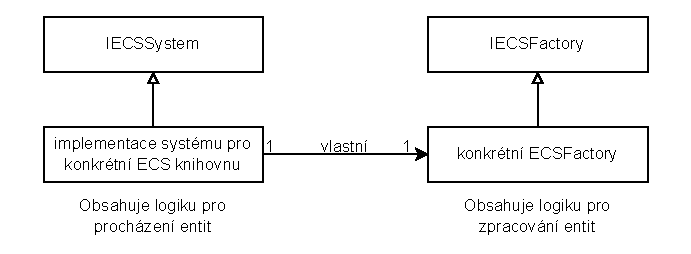
\includegraphics[width=0.8\linewidth]{img/abstract-layer-systems.pdf}
  \caption{Vztahy tříd souvisejících se systémy.}
  \label{fig:abstract-layer-systems}
\end{figure}

\texttt{IECSSystem} je rozhraní ze kterého dědí každý systém. Každá ECS knihovna poté poskytne svojí implementaci systému. Tyto implementace obsahují pouze logiku pro iteraci neboli procházení přes jednotlivé entity. Každá implementace systému bude vlastnit konkrétní \texttt{EntityProcessor} dědicí od \texttt{IEntityProcessor}. Jednotlivé \texttt{EntityProcessor} jsou zodpovědné za zpracování entit. Jednotlivé implementace rozhraní \texttt{IECSSystem} jsou generické typy, které přijímají typ entity procesoru a také typy komponent, které od entit vyžadují jako generické parametry.

Jako příklad si uvedeme třídu \texttt{ArchSystem<TEntityProcessor, TComponent>}. Jedná se o implementaci systému. Tento systém obsahuje logiku pro iteraci entit z ECS knihovny \textit{Arch}~\cite{Arch}. Příkladem konkrétního \texttt{EntityProcessor} je například třída \texttt{MovementSystem}, která řeší zpracování entit s komponentami \texttt{Position} a \texttt{Movement} a obsahuje logiku zodpovědnou za jejich pohyb.

Z pohledu hry jednotlivé implementace \texttt{EntityProcessor} představují samotné systémy, jelikož hra nekouká na to jak jsou entity iterovány a zajímá ji jenom samotná herní logika. Proto se kód, který pracuje s hrou odkazuje na \texttt{EntityProcessor} jako na systém. Ovšem z pohledu abstrakční vrstvy je nutné rozlišovat \texttt{System} jako typ, který obsahuje logiku pro iteraci entit a \texttt{EntityProcessor} jako typ, který obsahuje logiku pro zpracování entit. Autor si je vědom, že tyto pohledy mohou vést k matoucí terminologii, ovšem v kódu jsou již používány na příliš mnoho místech.

\subsection{ECSFactory}
\texttt{ECSFactory} je abstraktní třída. Typy, které z ní dědí jsou zodpovědné za tvorbu instancí související s abstrakční vrstvou. Vztah typů souvisejících s \texttt{ECSFactory} je možné vidět na obrázku~\ref{fig:abstract-layer-ecsfactory}.

\begin{figure}[!htb]
  \centering
  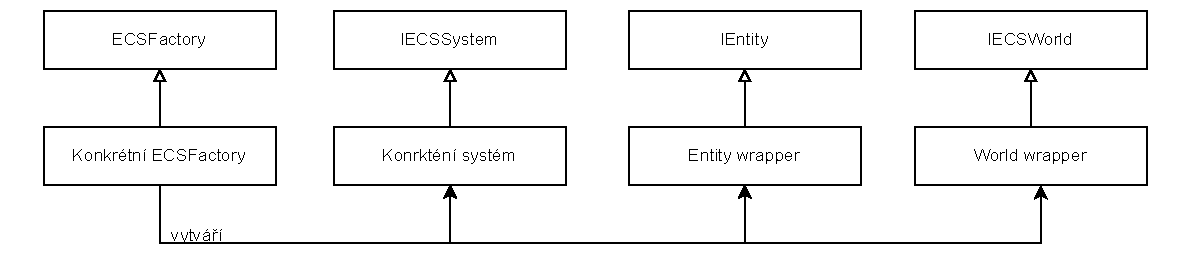
\includegraphics[width=1.0\linewidth]{img/abstract-layer-ecsfactory.pdf}
  \caption{Vztahy tříd souvisejících s \texttt{ECSFactory}.}
  \label{fig:abstract-layer-ecsfactory}
\end{figure}

Typ, který dědí od \texttt{ECSFactory} musí implementovat metody pro vyváření instancí wrapperu entity a wrapperu \textit{worldu}. Skrze konstruktor svému předku také předá typy jednotlivých systémů (tříd dědicích od \texttt{IECSSystem}). Wrapper entity je třída dědicí od rozhraní \texttt{IEntity} a je zodpovědná za přidávání a odebíraní komponent na dané entitě. Wrapper \textit{worldu} je třída dědicí od rozhraní \texttt{IECSWorld}. Tento wrapper implementuje metodu \texttt{Update}, která je zodpovědná za aktulizaci stavu \textit{worldu}.

\section{Hra}
\label{sec:game-impl}
Celá hra je reprezentována třídou \texttt{Game}, té je skrze konstruktor předána konkrétní instance \texttt{ECSFactory}. Jednotlivé instance \texttt{ECSFactory} reprezentují jednotlivé ECS knihovny a volba této instance představuje volbu ECS knihovny se kterou bude hra pracovat.

První herní stav je hře předán skrze metodu \texttt{SwitchState}. Samotná hra je spuštěna metodou \texttt{Run}.

\subsection{Herní stavy}
Celá hra se může skládat z několika herních stavů. Každý herní stav je reprezentován třídou dědicí od \texttt{GameState} a představuje herní obrazovku. Hra momentálně obsahuje pouze herní stav \texttt{LevelState}, který reprezentuje herní obrazovku obsahující gameplay, ale díky abstrakcí herních stavů by bylo snadné ji rozšířit například o herní obrazovku herního menu, nebo herní obrazovku s nastavením hry. Vztahy tříd souvisejících se třídou \texttt{GameState} lze vidět na obrázku~\ref{fig:game-state}.

\begin{figure}[!htb]
  \centering
  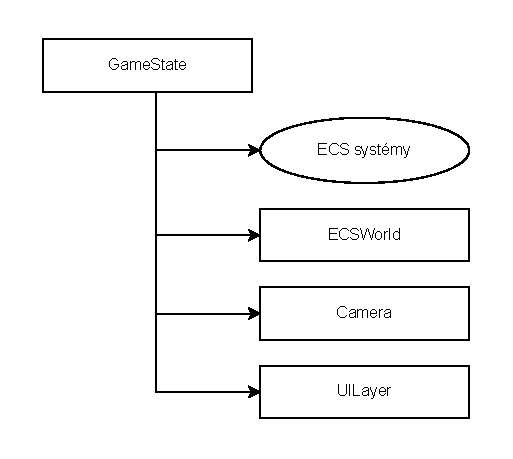
\includegraphics[width=0.5\linewidth]{img/game-state.pdf}
  \caption{Vztahy tříd souvisejících s \texttt{GameState}.}
  \label{fig:game-state}
\end{figure}

Každý herní stav obsahuje svoji instanci \texttt{ECSWorld}, která reprezentuje \textit{world} herního stavu. Tím pádem každý herní stav má svojí množinu entit. Dále má každý herní stav svoje systémy, kameru a instanci třídy \texttt{UILayer}, která spravuje prvky uživatelského rozhraní pro daný herní stav. Konkrétní herní stavy (instance tříd dědicích od \texttt{GameState}) jsou zodpovědné za vytváření svých entit, systémů a prvků uživatelského rozhraní.

V jeden moment může být aktivní pouze jeden herní stav. Ten lze zvolit za pomoci metody \texttt{SwitchState} na třídě \texttt{Game}. Vždy jsou aktivní pouze systémy v aktivním herním stavu.

\subsection{LevelState a herní svět}
\texttt{LevelState} je herní stav, který reprezentuje herní obrazovku obsahující samotný gameplay. Obrázek~\ref{fig:level-state} popisuje vztahy na této třídě.

\begin{figure}[!htb]
  \centering
  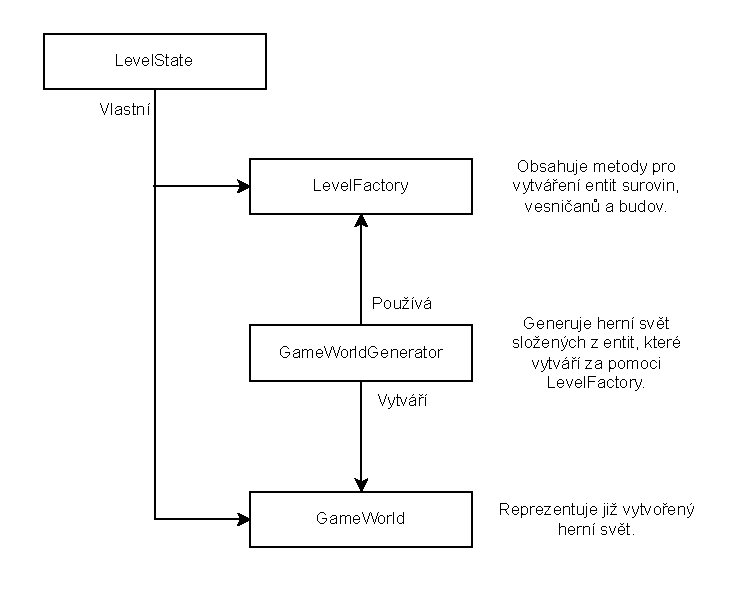
\includegraphics[width=0.7\linewidth]{img/level-state.pdf}
  \caption{Vztahy tříd souvisejících s \texttt{LevelState}.}
  \label{fig:level-state}
\end{figure}

Třída \texttt{LevelFactory}, obsahuje metody pro vytváření entit surovin, budov a vesničanů. Tu využívá třída \texttt{GameWorldGenerator} pro tvorbu entit z kterých generuje herní svět. Ta se krom vytváření samotného terénu stará také a počáteční rozpoložení surovin a vesnic. Výsledný vygenerovaný herní svět je poté reprezentován třídou \texttt{GameWorld}.

Pomocí třídy \texttt{GameWorld} lze získávat informace o herním světě. Je možné nalézt nejbližší surovinu určitého typu k dané pozici, nalézt cestu mezi dvěma body, nebo získat informace o terénu na dané pozici.

Na obrázku \ref{fig:game-world} lze vidět, že \texttt{GameWorld} obsahuje kd-strom pro každý typ suroviny. Pomocí této datové struktury lze efektivně nalézt nejbližší surovinu k dané pozici. Těmto kd-stromům se budeme více věnovat v sekci~\ref{sec:res-impl}. \texttt{GameWorld} v sobě také obsahuje dvourozměrnou mřížku s informacemi o terénu, která je používaná například pro hledání cest.

\begin{figure}[!htb]
  \centering
  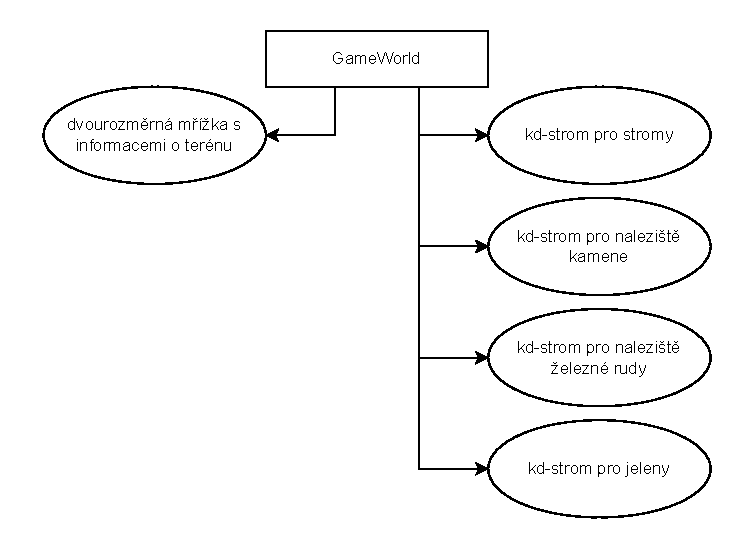
\includegraphics[width=0.8\linewidth]{img/game-world.pdf}
  \caption{Datové struktury obsažené v \texttt{GameWorld}.}
  \label{fig:game-world}
\end{figure}

Instance jednotlivých kd-stromů z obrázku~\ref{fig:game-world} jsou uchovávány v \texttt{Dictionary} uvnitř třídy \texttt{GameWorld}. Toto \texttt{Dictionary} mapuje typ suroviny (instanci třídy \texttt{ResourceType}) na konkrétní kd-tree. Díky tomuto \texttt{Dictionary} můžeme snadno získat kd-strom pro konkrétní typ suroviny.

\subsection{Assety}
Na obrázků~\ref{fig:asset-manager} lze vidět hierarchii tříd souvisejících s managementem assetů. \texttt{AssetManager<TAsset>} obsahuje společnou logiku pro nalezení a načtení assetů ze složky a pro správu slovníku ve kterém jsou uloženy načtené assety pro generický typ \texttt{TAsset}. Jednotlivý potomci této třídy poskytují implementace metody \texttt{Load}, pro načtení assetu konkrétního typu. I přesto, že hra momentálně obsahuje pouze assety pro textury a shadery, bylo by díky abstrakci asset managerů snadné hru rozšířit i o jiné typy assetů jako jsou například zvuky.

\begin{figure}[!htb]
  \centering
  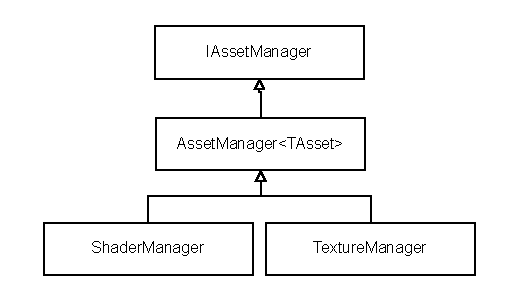
\includegraphics[width=0.6\linewidth]{img/asset-manager.pdf}
  \caption{Hierarchie dědičnosti tříd souvisejících s managementem assetů.}
  \label{fig:asset-manager}
\end{figure}

Všechny assety se nachází ve složce \texttt{Content}. Jednotlivé typy assetů mají poté v této složce svou podsložku. Textury se nacházejí v podsložce \texttt{Textures} a shadery v podsložce \texttt{Shaders}. Je nutné zmínit, že složka \texttt{Shaders} obsahuje již zkompilované shadery.

Veškeré instance rozhraní \texttt{IAssetManager} jsou uchovány ve třídě \texttt{Game}. Pomocí ní je také možné přistupovat ke konkrétním instancím (\texttt{ShaderManager} a \texttt{TextureManager}). Při inicializaci hry dojde k zavolání metody \texttt{LoadAll} na každé takové instanci. To vede k načtení všech assetů daného typu.

\subsection{Správa managed typů}
Vytváříme hru abychom jí později mohli používat pro měření výkonu ECS knihoven. Aby hru pro měření bylo možné použít, je klíčové, aby byla nezávislá na konkrétní ECS knihovně. Z toho důvodu hra namísto konkrétní ECS knihovny používá abstrakční vrstvu. V sekci~\ref{sec:components-analysis} jsme si zmínili, že jednotlivé komponenty v abstrakční vrstvě reprezentujeme jako struktury. Ovšem jedna z knihoven, které budeme měřit (konkrétně \textit{Svelto.ECS}~\cite{SveltoECS}), vyžaduje aby komponenty byli \textit{unmanaged typy}. V této sekci se zaměříme na to co to jsou \textit{unmanaged typy} a jak jsme tento problém vyřešili.

Definici \textit{unmanaged typů} lze nalézt ve článku \textit{Unmanaged types (C\# reference)}~\cite{Unmanagedtypes} od firmy \textit{Microsoft}. Ve článku se lze dočíst, že \textit{unmanaged typem} je každý z následujících datových typů:

\begin{enumerate}
  \item \texttt{sbyte}, \texttt{byte}, \texttt{short}, \texttt{ushort}, \texttt{int}, \texttt{uint}, \texttt{long}, \texttt{ulong}, \texttt{nint}, \texttt{nuint}, \texttt{char}, \texttt{float}, \texttt{double}, \texttt{decimal}, nebo \texttt{bool}.

  \item Jakýkoliv výčtový typ.
  
  \item Jakýkoliv typ ukazatele.

  \item Jakýkoliv tuple složený z \textit{unmanaged typů}.

  \item Jakákoliv uživatelem definovaná struktura, která obsahuje pouze fieldy \textit{unmanaged typů}.
\end{enumerate}

Naše komponenty jsou uživatelem definované struktury, tím pádem je pro nás klíčový poslední bod této definice. Konkrétně naše komponenty nesmí obsahovat jin0 fieldy, než fieldy \textit{unmanaged typů}. Ovšem v některých případech bychom takové fieldy potřebovali. Jedná se zejména o instance třídy \textit{IEntity} a jakékoliv pole nebo kolekce. Například entity vesničanů v naší hře obsahují \texttt{Villager} komponentu, ve které si uchovávají referenci na entitu vesnice do které spadají. Dalším příkladem je \textit{PathFollow} komponenta, která přidá entitě schopnost chodit po cestě, která je v této komponentě definována. Cesta je definována za pomocí pole pozic.

Pro řešení tohoto problému byli zavedeny manažery instancí \textit{managed typů}. Na obrázku~\ref{fig:unmanaged-data-managers} lze vidět hierarchii dědičnosti tříd souvisejících s těmito manažery. Prázdný interface \texttt{IManagedDataManager} slouží abychom mohli instance jednotlivých manažerů spolu ukládat do jedné kolekce. Od tohoto interface dědí abstraktní třída \texttt{ManagedDataManager<TManagedData>}, kde generický parametr \texttt{TManagedData} představuje \textit{managed typ}, jehož instance chceme spravovat. Od této třídy, dědí třídy, které se starají o správu konkrétních \textit{managed typů}.

\begin{figure}[!htb]
  \centering
  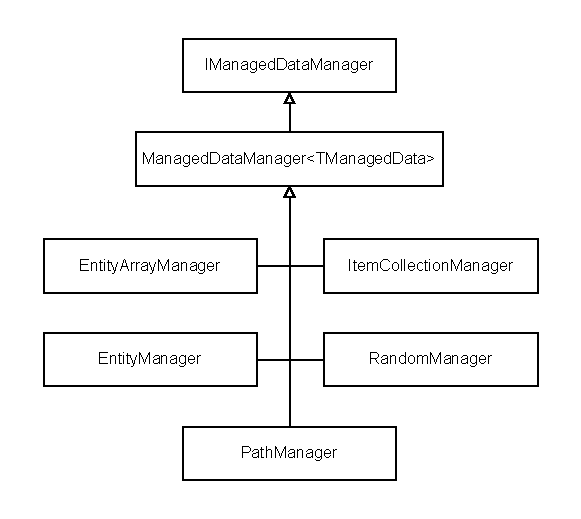
\includegraphics[width=0.6\linewidth]{img/managed_data_managers.pdf}
  \caption{Hierarchie dědičnosti tříd souvisejících se správou instancí \textit{managed typů}.}
  \label{fig:unmanaged-data-managers}
\end{figure}

Třída \texttt{ManagedDataManager<TManagedData>} obsahuje abstraktní metody pro vytvoření instancí spravovaného \textit{managed typu}. V jednotlivých manažerech jsou uchovávány spravované instance odpovídajícího \textit{managed typu}. Do manažera je možné instancí vložit nebo vytvořit novou instanci přímo uvnitř manažera. Obě tyto akce nám navrátí ID za pomoci, kterého lze k instancím daného \textit{managed typu} přistupovat. V našich komponentech namísto instancí těchto \textit{managed typů} uchováváme jejich ID.

V případě, že chceme odebrat danou komponentu, obsahující ID instance \textit{managed typu}, je nutné odpovídající instanci odebrat z manažera aby nedošlo k \textit{memory leaku}. V naší hře toto řešíme za pomoci \texttt{DeathSystem}, který řeší smrt entit. V případě smrti entity tento systém před odstranění dané entity zkontroluje zda na sobě daná entita nemá komponentu obsahující ID instance \textit{managed typu}. Pokud ano tak příslušnou instanci odebere z příslušného manažera.

Instance jednotlivých manažerů uchováváme ve třídě \texttt{Game}. Pomocí této třídy je možné k nim také přistupovat. Třídy pro typy jednotlivých manažerů je možné vidět na obrázku~\ref{fig:unmanaged-data-managers}.

\subsection{Uživatelské rozhraní}
Vztahy tříd souvisejících s uživatelským rozhraním je možné vidět na obrázku~\ref{fig:ui-layer}. Třída \texttt{UILayer} je zodpovědná za správu prvků uživatelského rozhraní pro jeden konkrétní herní stav. Každý prvek uživatelského rozhraní dědí od třídy \texttt{UIElement}. Hra momentálně obsahuje pouze jediný prvek uživatelského rozhraní a tím je minimapa (reprezentovaná třídou \texttt{Minimap}), ale je navržena tak aby bylo snadné ji rozšířit i o další prvky uživatelského rozhraní, jako jsou například labely, tlačítka, nebo action bar.

\begin{figure}[!htb]
  \centering
  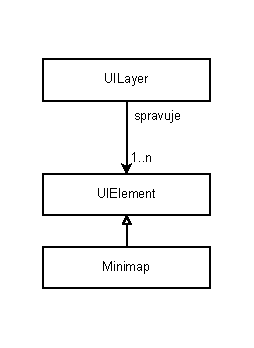
\includegraphics[width=0.35\linewidth]{img/ui-layer.pdf}
  \caption{Diagram vyobrazující vztahy tříd, které souvisejí s uživatelským rozhraním.}
  \label{fig:ui-layer}
\end{figure}

Mezi prvky uživatelského rozhraní existuje stromová hierarchie. Každý prvek může mít několik potomků. Jednotlivý potomci poté pracují s pozici relativní vůči svému rodiči.

\subsubsection{Minimapa}
Minimapa je reprezentována třídou \texttt{Minimap}, která dědí od \texttt{UIElement}. Pomocí minimapy chceme znázornit jak vypadá herní svět a jaká jeho část je momentálně viditelná kamerou. Jejím cílem je usnadnit hráčovi orientaci v herním světě.

Minimapa se skládá z mapy terénu, view framu a rámečku. Pro vykreslení mapy terénu používáme stejný fragment shader jako pro vykreslení terénu naší hry. Pouze použijeme jiné rozlišení a scale. Poté vykreslíme view frame, ten představuje výsek terénu, který hráč momentálně vidí skrze kameru. Pro jeho vykreslení si najdeme na jakou pozici v minimapě odpovídá umístění kamery a poté vykreslíme obdélníkový rámeček, který odpovídá rozměrům kamery naškálovaných podle velikosti minimapy. Aby nám view frame nepřesahoval hranice minimapy vykreslujeme jej s nastaveným \texttt{ScissorRectangle}. Jedná se o MonoGame nastavení, pomocí kterého lze provádět oříznutí. Na závěr kolem minimapy vykreslíme rámeček. Ten je reprezentován texturou.

\subsection{Herní data}
Mezi herní data patří informace o biomech, surovinách a předmětech. Herní data jsou immutable a lze k nim přistupovat globálně. Vztah tříd souvisejících s herními daty je možné vidět na obrázku \ref{fig:game-data}.

\begin{figure}[!htb]
  \centering
  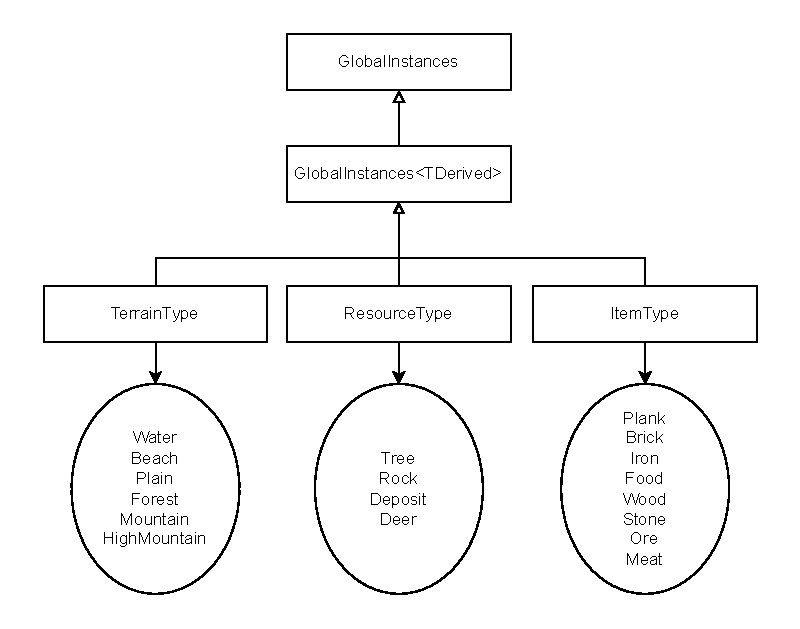
\includegraphics[width=0.7\linewidth]{img/game-data.pdf}
  \caption{Diagram vyobrazující třídy a důležité instance související s herními daty.}
  \label{fig:game-data}
\end{figure}

\texttt{GlobalInstances<TDerived>} je abstraktní třída, kde generický parametr \texttt{TDerived} může být pouze třída, která je jejím potomkem. \texttt{GlobalInstances<TDerived>} si za pomoci statiky interně ukládá všechny instance \texttt{TDerived} a umožňuje k nim globální přístup za pomoci jejich identifikátoru.

Jednotliví potomci třídy \texttt{GlobalInstances<TDerived>} představují jednotlivé typy herních dat, jako je například typ biomu (\texttt{TerrainType}), typ suroviny (\texttt{ResourceType}), nebo typ předmětu (\texttt{ItemType}). Tyto třídy obsahují informace o daném typu herních dat. Například typ biomu (\texttt{TerrainType}) obsahuje informaci o tom, zda je možné v daném biomu stavět a také informaci o tom, zda je možné v daném biomu chodit.

Je nutné, aby jednotlivý potomci třídy \texttt{GlobalInstances<TDerived>} měli privátní konstruktor, tím zaručíme, že nebude možné vytvářet nové instance mimo danou třídu. Všechny instance těchto potomků jsou definovány jako veřejné readonly statické fieldy přímo uvnitř těchto tříd.  Například herní data reprezentovaná třídou \texttt{TerrainType} obsahuje instance pro biom vody (\texttt{Water}), biom pláže (\texttt{Beach}), biom lesa (\texttt{Forest}) a další biomy. Na obrázku~\ref{fig:game-data} lze vidět vypsané jednotlivé instance jednotlivých typů herních dat.

Abstraktní třída \texttt{GlobalInstances} obsahuje pouze module initializer, pomocí kterého zavolá \texttt{RuntimeHelpers.RunClassConstructor} na každém neabstraktním typu, který od ní dědí. Tím máme zaručeno, že naše data jsou v čas vytvořené, jinak by k jejich vytvoření došlo až při prvním přístupu k jejich třídám a do té doby bychom k nim nemohli přistupovat skrze třídu \texttt{GlobalInstances<TDerived>}.

\subsection{Inventáře a předměty}
Na konci sekce~\ref{sec:game-world} jsme si uvedli jednotlivé typy předmětů, které jsou součástí naší hry. Jednotlivé předměty mohou mít vesničané ve svém inventáři (například pokud jej získali sklizením suroviny a nyní jej odnášejí, aby jej zpracovali). Dále jsou předměty skladovány ve skladišti. Vztahy tříd souvisejících z předměty je možné vidět na obrázku~\ref{fig:items}.

\begin{figure}[!htb]
  \centering
  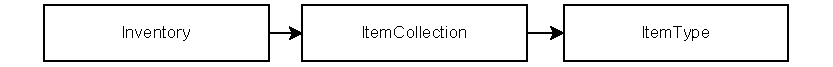
\includegraphics[width=0.8\linewidth]{img/items.pdf}
  \caption{Vztah tříd souvisejících s herními předměty.}
  \label{fig:items}
\end{figure}

Z minulé sekce víme, že instance třídy \texttt{ItemType} reprezentují jednotlivé typy předmětů. Každý typ předmětů má také svoje ID. Struktura \texttt{ItemCollection} reprezentuje kolekci předmětů. Uvnitř sebe má pole, kde jednotlivé prvky tohoto pole reprezentují počty předmětů uvnitř kolekce. Index každého prvku odpovídá ID daného typu předmětu. Například předmět \textit{prkno} má ID 0 a element z tohoto pole s indexem 0 odpovídá počtu prken uvnitř dané kolekce. Krom tohoto pole struktura \texttt{ItemCollection} také obsahuje pomocné metody pro manipulaci s kolekcemi předmětů.

Třída \texttt{Inventory} je komponenta. Entity s touto komponentou mají inventář do kterého mohou ukládat předměty. Tato třída obsahuje jediný field a tím je instance \texttt{ItemCollection}. Tuto komponentu na sobě krom entit vesničanů a skladišť mají také entity budov pro zpracování předmětů (například budova dřevorubce). Do tohoto inventáře přesouvají vesničané předměty pro zpracování a entita dané budovy pro zpracování surovin zde také ukládá produkt získaný zpracováním daného předmětu.

\subsection{Suroviny}
\label{sec:res-impl}
Jednotlivé suroviny jsou reprezentované jako entity. Komponenty, ze kterých jsou tyto entity složené a systémy, které tyto komponenty zpracovávají, je možné vidět na obrázku~\ref{fig:resource}. \texttt{RenderSystem} se stará o vykreslení entity. \texttt{Appearance} komponenta nese informaci o tom, jak entita vypadá a \texttt{Location} obsahuje informaci o tom kde se nachází. \texttt{DeathSystem} řeší logiku smrti dané entity, konkrétně v případě surovin dojde k jejich smrti v případě sklizení.

\begin{figure}[!htb]
  \centering
  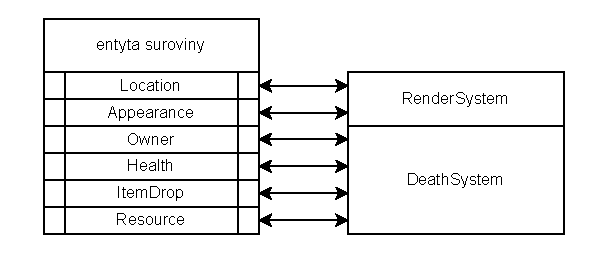
\includegraphics[width=0.8\linewidth]{img/resource.pdf}
  \caption{Entita suroviny s jejími komponentami a systémy, které tyto komponenty zpracovávají.}
  \label{fig:resource}
\end{figure}

Každá surovina má \texttt{Health} komponentu ve které má uloženou informaci o aktuálním počtu životů. Entita obsahující \texttt{DamageDealer} komponentu může zaútočit na entitu obsahující \texttt{Health} komponentu. Při tomto útoku se počet životů v příslušné \texttt{Health} komponentě sníží a pokud klesne na nulu, tak \texttt{DeathSystem} krom smazání mrtvé entity nahlédne zda zemřelá entita obsahuje \texttt{ItemDrop} komponentu. Pokud ano tak předměty definované v této komponentě převede do inventáře entity, které danou entitu zabila. Stejným způsobem funguje i sklízení surovin, kde útočící entitou je vesničan, který útočí na entitu dané suroviny a tím jí sklízí. Po jejím zabití neboli sklizení obdrží do svého inventáře příslušné předměty.

Suroviny na sobě mají také \texttt{Owner} komponentu. Ta obsahuje instanci typu dědicího od \texttt{IEntity}, která reprezentuje danou entitu. \texttt{DeathSystem} vyžaduje tuto komponentu aby mohl danou entitu smazat.

Jak již bylo zmíněno, existuje kd-tree pro každý typ suroviny. Jedná se o datovou strukturu pomocí které lze efektivně vyhledávat v prostoru. Entity jednotlivých surovin jsou uloženy v těchto kd-tree. Tyto kd-tree poté využívají vesničané, kteří v rámci svého povolání provádějí úlohu nalezení nejbližší suroviny daného typu. Pokud si vesničan rezervuje danou surovinu (začne pohyb směrem k ní a následně ji sklidí), dojde k odebrání této suroviny z příslušného kd-tree. Tím zamezíme tomu, že více vesničanů nebude sklízet stejnou entitu suroviny. Pro implementaci kd-tree používáme Nugget balíček \textit{KdTree}~\cite{KdTree}.

Dále je nutné zmínit, že \texttt{DeathSystem} pracuje nad všemi entitami s komponentami \texttt{Health} a \texttt{Owner}. V případě, že zemřelá entita má na sobě komponentu \texttt{Inventory} nebo komponentu \texttt{ItemDrop} tak převede dané předměty. A v případě, že zemřelá entita je vesničan a ten útočil na entitu s komponentou \texttt{Resource} (daná entita byla surovina), tak je nutné entitu vrátit do příslušného kd-tree.

Entita \textit{jelena} se od ostatních entit surovin liší. Její komponenty a systémy, které zpracovávají tyto komponenty je možné vidět na obrázku \ref{fig:deer}. Je možné nahlédnout, že oproti entitám ostatních surovin má entita \textit{jelena} navíc komponenty \texttt{Movement}, která přidává entitám schopnost chodit a \texttt{AnimalBehavior}. \texttt{AnimalBehaviorSystem} poté pracuje se všemi entitami s komponentami \texttt{Location}, \texttt{Owner}, \texttt{Movement} a \texttt{AnimalBehavior} a jeho hlavním úkolem je řídit chování zvířat, konkrétně jejich náhodný pohyb. Krom tohoto úkolu se tento systém stará také o aktulizaci pozice entit zvířat v příslušném kd-tree.

\begin{figure}[!htb]
  \centering
  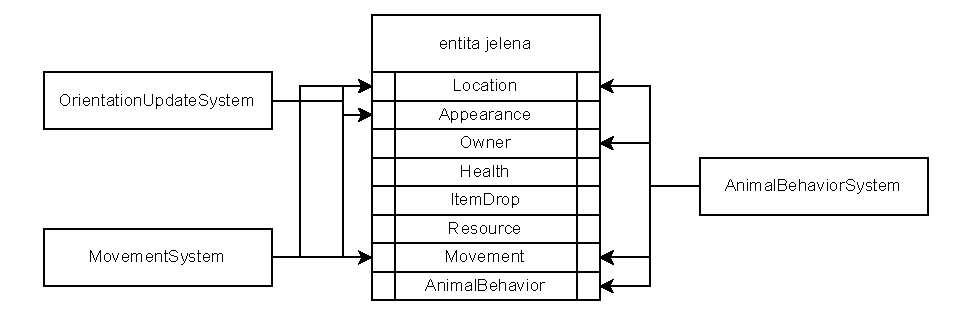
\includegraphics[width=1.0\linewidth]{img/deer.pdf}
  \caption{Entita jelena s jejími komponentami a systemy \texttt{AnimalBehaviorSystem}, \texttt{MovementSystem} a \texttt{OrientationUpdateSystem}.}
  \label{fig:deer}
\end{figure}

\texttt{MovementSystem} se stará o pohyb entit. Jak \texttt{MovementSystem} tak \texttt{AnimalBehaviorSystem} pracují s \texttt{Movement} komponentou, ale \texttt{AnimalBehaviorSystem} řídí jak se pohyb bude odehrávat a \texttt{MovementSystem} se stará o samotný pohyb. \texttt{OrientationUpdateSystem} aktualizuje orientaci entity. V závislosti na tom zda se entita pohybuje doleva nebo doprava tak převrátí texturu dané entity podle osy y aby její orientace odpovídala směru, ve kterém se pohybuje.

\subsection{Vesnice a vesničané}
Ze sekce~\ref{subsec:villages} víme, že v herním světě se budou nacházet vesničané a vesnice. Jednotlivé vesnice budou obsahovat budovy. Každá budova, každý vesničan a i samotná vesnice jsou reprezentované jako entity. V této sekci si tyto entity představíme.

\subsubsection{Vesničané}
Diagram s entitou vesničana je možné vidět na obrázku~\ref{fig:villager}. Krom vyobrazených systémů souvisí s vesničanem také \texttt{MovementSystem}, \texttt{DeathSystem}, \texttt{OrientationUpdateSystem} a \texttt{RenderSystem}. Tyto systémy byly popsány v minulé sekci a nyní se jim nebudeme věnovat.

\begin{figure}[!htb]
  \centering
  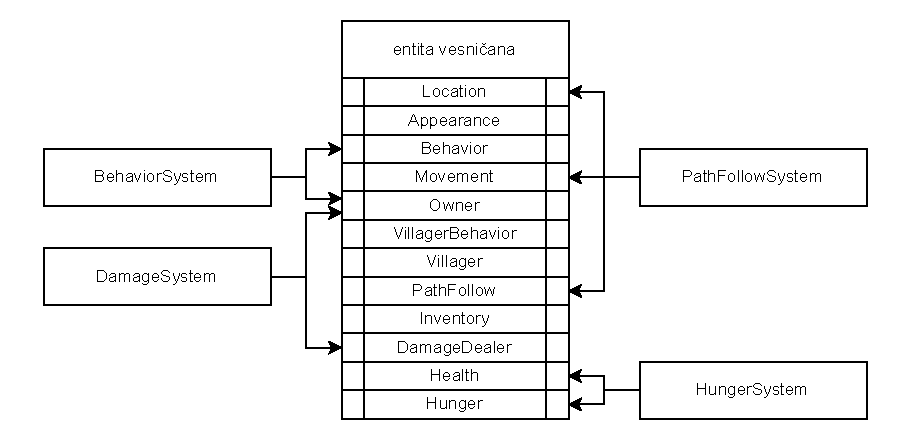
\includegraphics[width=1.0\linewidth]{img/villager.pdf}
  \caption{Entita vesničana s jejími komponentami a systemy \texttt{BehaviorSystem}, \texttt{PathFollowSystem}, \texttt{DamageSystem} a \texttt{HungerSystem}.}
  \label{fig:villager}
\end{figure}

Již zmiňovaný \texttt{DamageSystem} řeší logiku poškození. Z minulé sekce víme, že díky tomuto systému je vesničanům umožněno sklízet suroviny. \texttt{HungerSystem} řeší logiku hladovění. V \texttt{Hunger} komponentě je uložen aktuální stav hladovění vesničana. Tento stav neustále roste a pokud přesáhne určitou hranici, vesničan začne ztrácet životy. Pokud vesničan sní jídlo stav hladovění se nastaví na nulu.

\texttt{BehaviorSystem} se stará o chování vesničanů. Ze sekce~\ref{sec:ai} víme, že pro chování vesničanů používáme \textit{BehaviorTree}. Každý vesničan má právě jeden \textit{BehaviorTree} a \texttt{BehaviorSystem} pouze volá metodu \textit{Tick} na daném \textit{BehaviorTree}, která jej zpracovává.

Některé části z tohoto \textit{BehaviorTree} každého vesničana se starají o generování cest. Například pokud vesničan potřebuje dojít k entitě dané suroviny. Vygenerovaná cesta je poté uložena do \texttt{PathFollow} komponenty. O logiku chození po cestě se stará \texttt{PathFollowSystem}. Je nutné zmínit, že samotný pohyb vždy řeší \texttt{MovementSystem}, \texttt{PathFollowSystem} pouze nastavuje hodnoty v \texttt{Movement} komponentě na základě cesty uložené v \texttt{PathFollow} komponentě.

\subsubsection{Budovy}
Diagram entity budovy je možné vidět na obrázku~\ref{fig:building}. Vyobrazené komponenty má na sobě každá budova. V komponentě \texttt{Village} je uchovávaný odkaz na instanci vesnice do které budova spadá. Budova skladiště má na sobě navíc \texttt{Inventory} komponentu ve které ukládá suroviny, které vesnice vlastní. Hlavní budova oproti diagramu neobsahuje žádné dodatečné komponenty.

\begin{figure}[!htb]
  \centering
  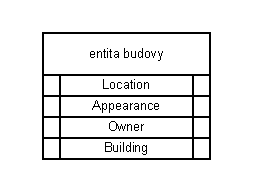
\includegraphics[width=0.4\linewidth]{img/building.pdf}
  \caption{Entita budovy s jejími komponentami.}
  \label{fig:building}
\end{figure}

Důležitým typem budov jsou budovy pro zpracování surovin. Diagram vyobrazující její komponenty a související systémy je možné vidět na obrázku~\ref{fig:res_building}. Je možné vidět, že oproti entitě z obrázku~\ref{fig:building} má budova pro zpracování surovin navíc komponenty \texttt{Inventory}, \texttt{ResourceProcessor} a \texttt{VillagerSpawner}.

\begin{figure}[!htb]
  \centering
  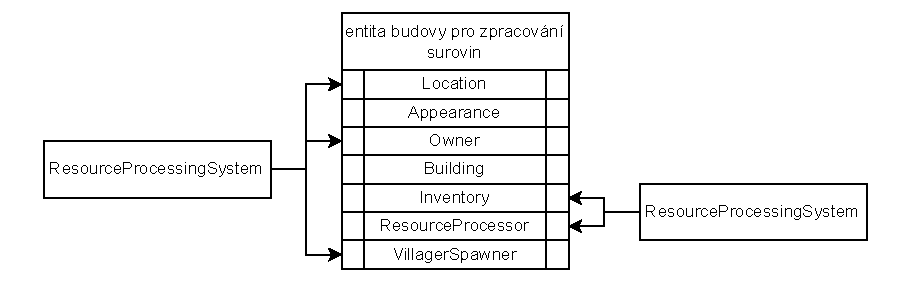
\includegraphics[width=1.0\linewidth]{img/resource_building.pdf}
  \caption{Entita budovy pro zpracování surovin s jejími komponentami a systémy \texttt{ResourceProcessingSystem} a \texttt{VillagerSpawningSystem}.}
  \label{fig:res_building}
\end{figure}

\texttt{VillagerSpawningSystem} je zodpovědný za vytváření nových vesničanů. Ke každé budově pro zpracování surovin je přidělen právě jeden vesničan a pokud tento vesničan zemře, tak se spustí odpočet. Po uplynutí tohoto odpočtu dojde k vytvoření nového vesničana. Při jeho vytvoření mu bude zkonstruován a přidělen \textit{BehaviorTree} a příslušná budova mu bude nastavena jako pracovní místo.

\texttt{ResourceProcessingSystem} se stará o logiku kolem zpracování surovin. Budovy pro zpracování surovin na sobě mají \texttt{Inventory} komponentu. \texttt{ResourceProcessingSystem} má na sobě nastavený recept a pravidelně nahlíží zda se v inventáři dané suroviny nacházejí požadované suroviny. Pokud ano, tak zahájí zpracování po jehož dokončení přemístí nově vytvořené předměty opět do inventáře. Z něj je může vesničan převzít a odnést do skladiště.

\subsubsection{Vesnice}
Každá vesnice je entita, která obsahuje komponenty \texttt{Location}, \texttt{Village} a \texttt{Owner}. \texttt{VillageBuildingSystem} se stará se stavění budov v dané vesnici. Má v sobě uloženou stavební frontu budov, kde pro každou budovu má také její cenu. Ve \texttt{Village} komponentě jsou uchovávány odkazy na jednotlivé entity budov, které se ve vesnici nacházejí. Jakmile \texttt{VillageBuildingSystem} zjistí, že vesnice má dostatek surovin na další budovu ze stavební fronty, vytvoří pro ni entitu a přidá na vytvořenou entitu odkaz do \texttt{Village} komponenty.

Klíčovou částí při vytváření entity budovy je volba pozice kde se entita má vytvořit. Nechceme aby budovy byli umístěny v biomech kde nelze stavět a také nechceme aby se nacházeli moc blízko nebo moc daleko od ostatních budov. Pro volbu pozice budov je zvolena konstantní minimální a maximální vzdálenost. Tyto vzdálenosti udávají v jakém rozmezí se mohou nové budovy od již postavených budov objevit.

Pro volbu pozice byl použit přímočarý algoritmus. Jako první se vybere náhodná již postavená budova a vezme se její pozice. Poté se kolem této pozice vytvoří prstenec s rozměry podle konstantní minimální a maximální vzdálenosti. V tomto prstenci se poté vybere náhodná pozice. Na závěr se zkontroluje zda je možné na této pozici stavět a pokud ano tak je tato pozice vybrána jako pozice pro novou budovu. Pokud na dané pozici není možné stavět tak se celý algoritmus zopakuje.

\section{Měření}
\label{benchmark-implementation}
Měření je druhým C\# projektem (\texttt{WorldSimulator.Benchmarks.csproj}) našeho C\# solution. S použitím naší hry měří výkon jednotlivých ECS knihoven. V sekci~\ref{benchmark-framework} jsme se rozhodli, že pro toto měření použijeme \textit{BenchmarkDotNet}. Celé měření se dělí na dvě fáze a to přípravy a samotného měření.

Pro měření máme definované následující konstanty:

\begin{enumerate}
  \item \texttt{seed}: Seed pro generování náhodných čísel. Stejným seedem pro každé měření zajistíme konzistentnost.

  \item \texttt{deltaTime}: Čas v sekundách. Tento čas používáme pro odsimulovaní jednoho kroku naší hry (jedné iterace \textit{game loop}, který byl přiblížen v sekci~\ref{game-loop}).

  \item \texttt{setupIterationCount} Udává počet kroků odsimulování naší hry během fáze přípravy.

  \item \texttt{benchmarkIterationCount}: Udává počet kroků odsimulování hry během fáze měření.
\end{enumerate}

V C\# projektu (\texttt{WorldSimulator.Benchmarks.csproj}) máme definovaný test reprezentovaný třídou \texttt{ECSBenchmarks}. Tento test obsahuje jediný vstupní parametr a tím je \texttt{ECSFactoryType} typu \texttt{Type}. Tímto parametrem jsou předávány typy dědicí od \texttt{ECSFactory}, které reprezentují jednotlivé ECS knihovny.

Během fáze přípravy nejprve zkonstruujeme konkrétní \texttt{ECSFactory}. Poté vytvoříme novou instanci naší hry (třídy \texttt{Game}) a odsimulujeme jeden její snímek za pomocí \texttt{RunOneFrame}, tím zaručíme, že hra bude inicializována. Poté v cyklu voláme metodu \texttt{UpdateOnce}, která vykoná jednu iteraci \textit{game loop} naší hry. Počet opakování tohoto cyklu udává konstanta \texttt{setupIterationCount}.

Během fáze měření používáme tu samou instanci hry vytvořené během fáze přípravy. Na této instanci v cyklu opět zavoláme metodu \texttt{UpdateOnce}. Počet opakování tohoto cyklu je dán konstantou \texttt{benchmarkIterationCount}.

% \newpage
% \null










% \subsection{Herní mechaniky}
% Implementace jednotlivých herních mechanik je možné najít v jednotlivých systémech (myšleno typech dědicích od \texttt{IEntityProcesor}) a komponentách. Všechny komponenty se nacházejí ve jmenném prostoru \texttt{WorldSimulator.Components}. Všechny systémy v \texttt{WorldSimulator.Systems}.

% Některé systémy se zabývají vykreslováním hry. Tyto systémy se reprezentují stejným způsobem jako běžné systémy, akorát k jejich vytvoření dojde v metodě \texttt{GameState.CreateRenderSystems} namísto metody \texttt{GameState.CreateSystems}, ve které se běžně vytvářejí systémy.




















% \begin{enumerate}
%     \item \textbf{\texttt{IECSSystem}:} Jedná se o rozhraní. Instance typů, které implementují toto rozhraní, představují kompletní systém. Tyto typy obsahují logiku pro iteraci přes jednotlivé entity. O zpracování jednotlivých entit se stará \texttt{EntityProcessor}. Každá instance kompletního systému má na sobě právě jeden \texttt{EntityProcessor}. Například \texttt{ArchSystem<TEntityProcessor, TComponent>} je systém, který obsahuje logiku pro procházení entit z ECS knihovny \textit{Arch}~\cite{Arch}.

%     \item \textbf{\texttt{IEntityProcesor}:} Jedná se o rozhraní, které ma na sobě klíčovou metodu \texttt{Process}. Typy, které implementují toto rozhraní obsahují herní logiku, která zpracovává jednotlivé entity. Například \verb|MovementSystem| ve své metodě \verb|Process| zpracuje pohyb pro danou entitu.

%     Z pohledu hry jednotlivé implementace \textit{EntityProcessor} představují samotné systémy, jelikož hra nekouká na to jak jsou entity iterovány a zajímá je jenom samotná herní logika. Proto se kód, který pracuje s hrou odkazuje na \texttt{EntityProcessor} jako na systém. Ovšem z pohledu abstrakční vrstvy je nutné rozlišovat \texttt{System} jako typ, který obsahuje logiku pro iteraci entit a \texttt{EntityProcessor} jako typ, který obsahuje logiku pro zpracování entit. Autor si je vědom, že tyto pohledy mohou vést k matoucí terminologii, ovšem v kódu jsou již používány na příliš mnoho místech.

%     \item \textbf{\texttt{}:} Jedná se o rozhraní. Typy, které implementují toto rozhraní definují logiku pro vytváření entity a \textit{world} dané implementace abstrakční vrstvy. Pomocí instancí těchto typů je také možné vytvářet instance kompletních systémů. Tyto typy také reprezentují celou jednu implementaci abstrakční vrstvy.

%     \item \textbf{\texttt{IECSWorld}:} Jedná se rozhraní. Typy, které implementují toto rozhraní, představují \textit{world} pro danou ECS knihovnu. Jelikož pro velkou část ECS knihoven typy, které implementovali toto rozhraní, vypadali identicky, byl zaveden typ \texttt{BasicECSWorld}. Tento typ lze použít pro většinu ECS knihoven.

%     \item \textbf{\texttt{IEntity}:} Jedná se o rozhraní. Typy, které implementují toto rozhraní představují entitu v konkrétní ECS knihovně.

%     \item \textbf{\texttt{ComponentAttribute}:}. Některé ECS knihovny potřebují před spuštěním hry vědět o typech všech komponent, které budou ve hře používány. Proto je typ jakékoliv komponenty označen tímto atributem a v případě, že některá ECS knihovna bude potřebovat znát typy jednotlivých komponent, může si skrze reflexi najít všechny typy s tímto atributem.
% \end{enumerate}






% Popis a provázanost členů. Co musí ECS knihovna implementovat. V jakém je to namespace.

% \section{Hra}

% Popis a provázanost  členů.

% \subsection{Herní svět}












% V této kapitole si představíme klíčové a zajímavé části implementace naší hry. Pro více detailů o implementaci je možné nahlédnout do kódu, který obsahuje dokumentační komentáře.

% Pro tvorbu hry byl použit MonoGame framework~\cite{MonoGame}, ovšem základní MonoGame nemá podporu pro compute shadery, které jsme využili pro řešení problému s vyhledávání cesty v podsekci~\ref{subsection:path-finding}. Z toho důvodu byl použit fork~\cite{MonoGameCptMax}, který tuto podporu nabízí.

% \section{Abstrakční vrstva}
% \label{sec:abstract-layer}
% Některé typy z abstrakční vrstvy jsme si již představili v sekci \ref{section:abstract-layer-analysis}. Pro připomenutí si nyní tyto typy lehce představíme znovu a zároveň si popíšeme další důležité typy z abstrakční vrstvy:

% \begin{enumerate}
%     \item \textbf{\texttt{IECSSystem}:} Jedná se o rozhraní. Instance typů, které implementují toto rozhraní, představují kompletní systém. Tyto typy obsahují logiku pro iteraci přes jednotlivé entity. O zpracování jednotlivých entit se stará \texttt{EntityProcessor}. Každá instance kompletního systému má na sobě právě jeden \texttt{EntityProcessor}. Například \texttt{ArchSystem<TEntityProcessor, TComponent>} je systém, který obsahuje logiku pro procházení entit z ECS knihovny \textit{Arch}~\cite{Arch}.

%     \item \textbf{\texttt{IEntityProcesor}:} Jedná se o rozhraní, které ma na sobě klíčovou metodu \texttt{Process}. Typy, které implementují toto rozhraní obsahují herní logiku, která zpracovává jednotlivé entity. Například \verb|MovementSystem| ve své metodě \verb|Process| zpracuje pohyb pro danou entitu.

%     Z pohledu hry jednotlivé implementace \textit{EntityProcessor} představují samotné systémy, jelikož hra nekouká na to jak jsou entity iterovány a zajímá je jenom samotná herní logika. Proto se kód, který pracuje s hrou odkazuje na \texttt{EntityProcessor} jako na systém. Ovšem z pohledu abstrakční vrstvy je nutné rozlišovat \texttt{System} jako typ, který obsahuje logiku pro iteraci entit a \texttt{EntityProcessor} jako typ, který obsahuje logiku pro zpracování entit. Autor si je vědom, že tyto pohledy mohou vést k matoucí terminologii, ovšem v kódu jsou již používány na příliš mnoho místech.

%     \item \textbf{\texttt{}:} Jedná se o rozhraní. Typy, které implementují toto rozhraní definují logiku pro vytváření entity a \textit{world} dané implementace abstrakční vrstvy. Pomocí instancí těchto typů je také možné vytvářet instance kompletních systémů. Tyto typy také reprezentují celou jednu implementaci abstrakční vrstvy.

%     \item \textbf{\texttt{IECSWorld}:} Jedná se rozhraní. Typy, které implementují toto rozhraní, představují \textit{world} pro danou ECS knihovnu. Jelikož pro velkou část ECS knihoven typy, které implementovali toto rozhraní, vypadali identicky, byl zaveden typ \texttt{BasicECSWorld}. Tento typ lze použít pro většinu ECS knihoven.

%     \item \textbf{\texttt{IEntity}:} Jedná se o rozhraní. Typy, které implementují toto rozhraní představují entitu v konkrétní ECS knihovně.

%     \item \textbf{\texttt{ComponentAttribute}:}. Některé ECS knihovny potřebují před spuštěním hry vědět o typech všech komponent, které budou ve hře používány. Proto je typ jakékoliv komponenty označen tímto atributem a v případě, že některá ECS knihovna bude potřebovat znát typy jednotlivých komponent, může si skrze reflexi najít všechny typy s tímto atributem.
% \end{enumerate}

% \section{Páteřní kód}
% Páteřní kód naší hry se skládá z následujících tříd:

% \begin{enumerate}
%     \item \textbf{\texttt{Game}:} Tato třída představuje samotnou hru. Dědí od třídy \texttt{Microsoft.Xna} \texttt{.Framework.Game} a přetěžuje od ní klíčové metody \verb|Update| a \verb|Draw|. Tato třída přijímá skrze konstruktor instanci typu, který implementuje rozhraní \texttt{}. Pomocí této instance je možné zvolit konkrétní implementaci abstrakční vrstvy neboli konkrétní ECS knihovnu se kterou bude hra pracovat.

%     \item \textbf{\texttt{GameState}:} Abstraktní třída \verb|GameState| představuje herní obrazovku. Herní obrazovky mohou být například Menu, Nastavení, nebo Level. I přesto, že naše hra obsahuje pouze jednu herní obrazovku, díky této třídě by bylo jednoduché do hry výše zmíněné herní obrazovky přidat.

%     \verb|GameState| si v sobě uchovává všechny systémy, které jsou rozděleny do dvou kolekcí. První je kolekce \verb|renderSystems|, která obsahuje všechny systémy, které řeší vykreslování. Druhá kolekce je \verb|systems|, která obsahuje všechny ostatní systémy.

%     \verb|GameState| má na sobě definované dvě klíčové metody a to \verb|Update| a \verb|Draw|. V \verb|Update| se zpracují všechny systémy z kolekce \verb|systems| a v \verb|Draw| se zpracují všechny systémy z kolekce \verb|renderSystems|.

%     \texttt{Game} má v jeden moment aktivní pouze jedenu herní obrazovku pro kterou ve své metodě \texttt{Update} volá \texttt{Update} na této herní obrazovce a ve své metodě \texttt{Draw} volá \texttt{Draw} na této herní obrazovce.

%     Mezi důležité členy, které \verb|GameState| obsahuje patří:

%     \begin{enumerate}
%         \item \textbf{\texttt{ECSWorld}:} Tento člen implementuje rozhraní \verb|IECSWorld| a představuje správce všech entit a komponent uvnitř jednoho \verb|GameState|.
%         \item \textbf{\texttt{Camera}:} Představuje herní kameru.
%         \item \textbf{\texttt{UILayer}:} Jedná se o správce prvků uživatelského rozhraní uvnitř jednoho \verb|GameState|.
%     \end{enumerate}

%     \verb|GameState| obsahuje metodu \verb|Initialize| ve které jsou volány abstraktní metody \verb|CreateEntities|, \verb|CreateSystems|, \verb|CreateRenderSystems| a \verb|CreateUI|, pomocí kterých jednotlivý potomci vytvářejí své entity, systémy a prvky uživatelského rozhraní.

%     \item \textbf{\texttt{LevelState}:} Třída \verb|LevelState| dědí od třídy \verb|GameState| a reprezentuje herní obrazovku, která obsahuje samotný level.

%     \item \textbf{\texttt{LevelFactory}:} Třída \verb|LevelFactory| obsahuje metody pro vytváření jednotlivých entit, která jsou používané v \verb|LevelState|.
% \end{enumerate}

% \section{Herní svět}
% Herní svět je reprezentován třídou \verb|GameWorld|. Tato třída obsahuje grid s informacemi o terénu, který je použit pro hledání cest. Do herního světa je možné přidávat suroviny skrze metodu \verb|AddResource|. Je také možné se dotazovat na informace ohledně terénu na konkrétní pozici v herním světě skrze metody \verb|GetTerrain|, \verb|CanWalkAt|, \verb|CanBuildAt|.

% O generování herního světa se stará třída \verb|GameWorldGenerator|. Při generování světa se nejprve vygeneruje samotný terén, poté dojde ke generování surovin a následně ke generování vesnic.

% Pro generování světa používáme dva shadery, konkrétně fragment shader pro vykreslování terénu, definovaný v souboru \textit{terrainDraw.fx} a compute shader pro generování dvourozměrného pole, které se používá pro hledání cest, definovaný v souboru \textit{terrainGen.fx}. Oba shadery využívají společnou část definovanou v souboru \textit{terrain.fx}.

% Společná část definovaná v souboru \textit{terrain.fx} je zodpovědná za generování terénu. Pro generování terénu je použit simplexův šum na jehož generování je využita knihovna lygia~\cite{lygia}. Pomocí simplexova šumu je vygenerována výšková mapa, která je poté namapována v příslušné biomy. Ve společné části jsou definované dvě důležité funkce a to \verb|CalcNoise|, která spočítá výšku pro specifikovanou pozici a \verb|GetTerrain|, která přijme výšku a na základě ní navrátí informace o daném biomu, který je pro tuto výšku mapován.

% Compute shader definovaný v souboru \textit{terrainGen.fx} přijímá jako vstupní parametry velikost herního světa a vzdálenost mezi jednotlivými body, které budou samplovány do již zmiňovaného 2D pole (viz sekce \ref{subsection:path-finding}). Mezi výstupy patří dva důležité buffery. Prvním je \verb|terrainBuffer|, který pro každý bod v gridu obsahuje identifikátor příslušného terénu. Druhým je \verb|resourceBuffer|, který obsahuje pozice na kterých bude vygenerována surovina.

% Fragment shader definovaný v souboru \textit{terrainDraw.fx} je zodpovědný za vykreslení oblasti z herního světa. Mezi jeho vstupní parametry patří velikost světa, velikost okna, přiblížení kamery a pozice kamery. Tento shader je použit kromě vykreslování samotného herního světa také k vykreslení minimapy.

% O samotné vykreslování herního světa se stará \texttt{TerrainRenderSystem}, který pro vykreslení volá fragment shader definovaný v souboru \textit{terrainDraw.fx}.

% \section{Herní data a jejich reprezentace}
% Pro reprezentaci některých dat v naší hře, může být užitečné mít zavedené datové typy, pro které budeme mít globální přístup ke každé instanci těchto typů. Mezi tyto data mohou patřit například suroviny (třída \texttt{ResourceType}), předměty (třída \texttt{ItemType}), nebo biomy (třída \texttt{TerrainType}).

% Pro reprezentaci těchto dat je zavedena třída \texttt{GlobalInstances}, která jako generický argument \texttt{TDerived} přijímá typ, který od této třídy dědí. Tato třída má interní statickou kolekci, ve které jsou uloženy všechny vytvořené instance třídy \texttt{TDerived}. Třída \texttt{GlobalInstances} je také zodpovědná za generování číselného identifikátoru pro každou instanci \texttt{TDerived}. Tento identifikátor slouží zároveň jako index dané instance. Konkrétní instanci lze získat skrze metodu \texttt{Get}, která navrátí instanci podle specifikovaného indexu.

% Jednotlivé typy, které dědí od \texttt{GlobalInstances} mají privátní konstruktor a všechny své instance definují přímo v sobě jako veřejné readonly statické členy.

% Následující kód je definicí surovin z naší hry a slouží jako příklad použití \texttt{GlobalInstances}:

% \begin{verbatim}
% /// <summary>
% /// Represent a type of a natural resource, which can
% /// be harvested to obtain items.
% /// </summary>
% internal sealed class ResourceType
%   : GlobalInstances<ResourceType>
% {
%   /// <summary>
%   /// The item obtained upon harvesting the resource.
%   /// </summary>
%   public ItemType HarvestItem { get; init; }
%   /// <summary>
%   /// The number of items obtained upon harvesting
%   /// the resource.
%   /// </summary>
%   public int HarvestQuantity { get; init; }
%   /// <summary>
%   /// How much time it takes to harvest the resource
%   /// in seconds.
%   /// </summary>
%   public float HarvestTime { get; init; }
%   private ResourceType() : base() { }
%   public readonly static ResourceType Tree = new()
%   {
%     HarvestItem = ItemType.Wood,
%     HarvestQuantity = 1,
%     HarvestTime = 3.0f,
%   };
%   public readonly static ResourceType Rock = new()
%   {
%     HarvestItem = ItemType.Stone,
%     HarvestQuantity = 1,
%     HarvestTime = 5.0f,
%   };
%   public readonly static ResourceType Deposit = new()
%   {
%     HarvestItem = ItemType.Ore,
%     HarvestQuantity = 1,
%     HarvestTime = 7.0f,
%   };
%   public readonly static ResourceType Deer = new()
%   {
%     HarvestItem = ItemType.Meat,
%     HarvestQuantity = 1,
%     HarvestTime = 9.0f,
%   };
% }
% \end{verbatim}

% \section{Herní mechaniky}
% Implementace jednotlivých herních mechanik je možné najít v jednotlivých systémech (myšleno typech dědicích od \texttt{IEntityProcesor}) a komponentách. Všechny komponenty se nacházejí ve jmenném prostoru \texttt{WorldSimulator.Components}. Všechny systémy v \texttt{WorldSimulator.Systems}.

% Některé systémy se zabývají vykreslováním hry. Tyto systémy se reprezentují stejným způsobem jako běžné systémy, akorát k jejich vytvoření dojde v metodě \texttt{GameState.CreateRenderSystems} namísto metody \texttt{GameState.CreateSystems}, ve které se běžně vytvářejí systémy. Za implementaci obou těchto metod jsou zodpovědní potomci třídy \texttt{GameSystem}.

% \section{Vesnice a vesničané}
% Jednotlivé vesnice jsou reprezentovány jako entity. Tyto entity na sobě mají \texttt{Village} komponentu, ve které si uchovávají seznam svých budov.

% Budovy jsou také reprezentovány jako entity. Entity budov na sobě mají \texttt{Building} komponentu, ve které si uchovávají entitu vesnice, do které spadají.

% Budovy pro zpracování surovin na sobě navíc mají \texttt{ResourceProcessor} komponentu. Tyto budovy se starají o zpracování surovin podle daného receptu, který mají uložen v této komponentě. Mechaniku pro zpracování surovin řeší \texttt{ResourceProcessingSystem}.

% Budovy pro zpracování surovin mají na sobě také \texttt{VillagerSpawner} komponentu. Ta je společně s \texttt{VillagerSpawningSystem} zodpovědná za mechaniku  vesničanů. Tato komponenta v sobě uchovává informace o tom jak dlouho trvá než dojde ke spawnutí vesničana a o profesi, která bude spawnutému vesničanovi přidělena. V případě, že vesničan zemře, začne odpočet a po jeho ukončení dojde ke spawnutí nového vesničana.

% village building system

% villagers

% \xxx{TODO}





























% \chapter{Popis implementace}
% V této kapitole si blíže představíme implementaci naší hry.

% \section{Abstrakce}
% Prvně si rozebereme jak vypadá páteřní kód naší hry.

% % Game, GameState, LevelState, Factory, LevelFactory

% Nyní si přibližme naší abstrakční vrstvu Abstract.ECS.

% % \xxx{Code base}
% % \\
% % \xxx{Abstract.ECS layer}

% \section{Herní svět}
% Herní svět je reprezentován třídou GameWorld.

% O generování herního světa se stará třída GameWorldGenerator.

% Rozeberme si co jsou to vlastně shadery.

% Naše hra používá dva shadery.

% % \xxx{GameWorld}
% % \\
% % \xxx{GameWorldGenerator}
% % \\
% % \xxx{Shaders}

% \section{Herní data a jejich reprezentace}

% Pro správu herních dat, slouží třída GlobalInstances.

% % co jsou herni data, co trida dela

% % \xxx{Data - biomes, items, and resources}

% \section{Systémy a komponenty}

% Následující seznam obsahuje a popisuje všechny herní systémy a komponenty.